\subsection{Second Experience}

\subsubsection{Python UDP Implementation (Loopback)}

After setting up a Python environment and running the provided scripts, we got
the following output:

\begin{figure}[htbp]
	\centering
	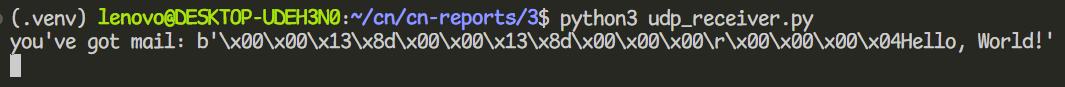
\includegraphics[width=1\linewidth]{img/second_exp/1.png}
	\caption{Receiver Output}\label{fig:2_1}
\end{figure}

\begin{figure}[htbp]
	\centering
	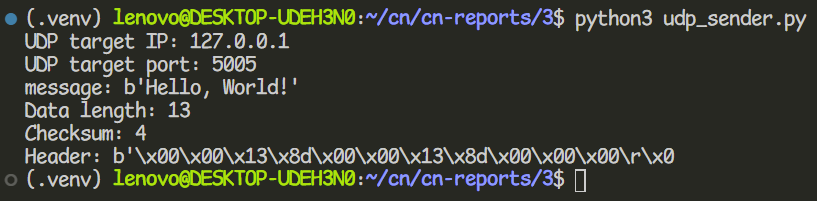
\includegraphics[width=1\linewidth]{img/second_exp/2.png}
	\caption{Sender Output}\label{fig:2_2}
\end{figure}

We can see that the received header matches the data sent by the sender, and
the IP is 127.0.0.1 as we were listening to that specific ip-port combination.

To further analyze the UDP package, we opened Wireshark and looked for the UDP
package.

\begin{figure}[htbp]
	\centering
	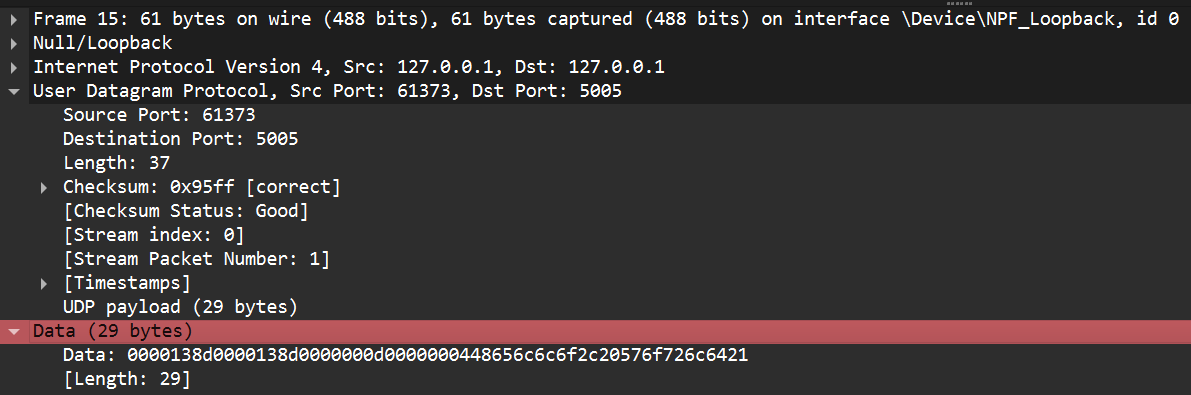
\includegraphics[width=1\linewidth]{img/second_exp/3.png}
	\caption{}\label{fig:2_3}
\end{figure}

The source port is 61373, which can be interpreted as a private port.
Destination port is 5005.

If we were to try and send the UDP packet to a different PC, we would need to:

\begin{itemize}
	\item be on the same network
	\item open port 5005 on the receiver PC (firewall might mess it up)
	\item change the target ip address in the python file
\end{itemize}

We also wanted to compare checksum values, and analyzed a different packet for
such task.

\begin{figure}[htbp]
	\centering
	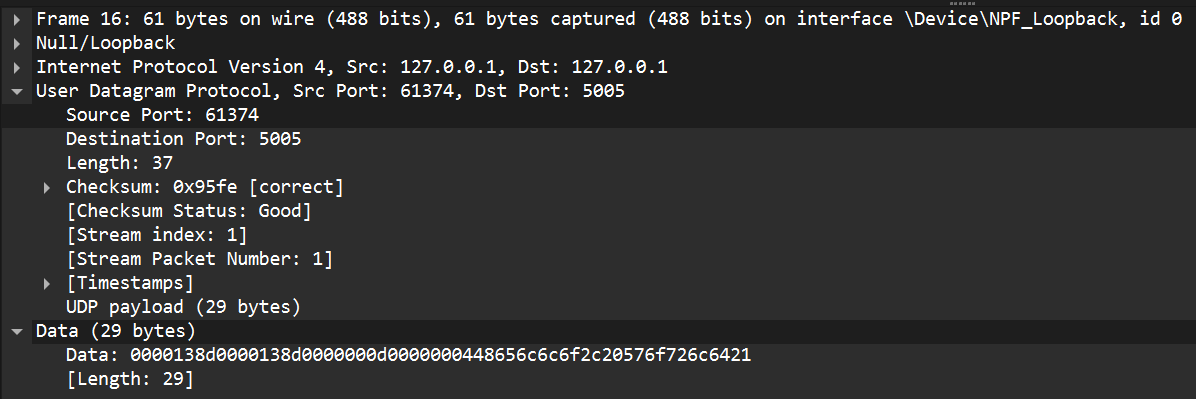
\includegraphics[width=1\linewidth]{img/second_exp/4.png}
	\caption{}\label{fig:2_4}
\end{figure}

The checksums differ by one byte. The first one is \texttt{Ox95ff}, while the
second packet shows a checksum with the value \texttt{0x95fe}. The checksums
were calculated and validated correctly, as displayed by Wireshark.

The 128 TTL value is set by Windows for outgoing IP packets, and as it never
leaves the PC, its TTL never changes (no hostname resolution).

The Wireshark packet was identified as UDP due to the port number. This is also
feasible for identifying application-layer protocol packets. Protocols like DNS
and DHCP use well-known ports (53 and 67/68). This method, however, does not
always work. After a bit of googling, we found out that Wireshark might resort
to heuristics when dealing with unrecognized packets.

Finally, we wanted to see what would happen if our sender script used a
non-routable or invalid IP address. We modified the \texttt{sender.py} script
to use the address \texttt{192.0.2.1} instead of \texttt{127.0.0.1}. The
receiver script was also modified. Wireshark detected no loopback packets, and
the receiver output was the following:

\begin{figure}[htbp]
	\centering
	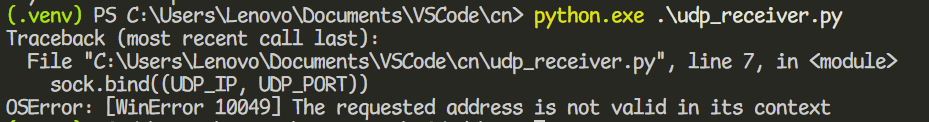
\includegraphics[width=1\linewidth]{img/second_exp/5.png}
	\caption{Receiver Output with invalid IP}\label{fig:2_5}
\end{figure}

A short research indicates that \texttt{192.0.2.1} is not a valid IP address,
and is reserved for use in documentation and code examples~\cite{rfc5735}.

\subsubsection{Python UDP Implementation (P2P)}
% TODO: info paca

